\documentclass{llncs}

\usepackage{graphicx}
%
\usepackage{geometry} % to change the page dimensions
\usepackage{multirow}
\usepackage{subfigure}


\geometry{a4paper}

\begin{document}


\title{Implementaci\'on de un Sistema Recuperaci\'on de Informaci\'on utilizando Redes Neuronales}

\author{Andy Gonz\'alez Pe\~na, Juan Eray \'Alvarez Hern\'andez}

\institute{MATCOM, Universidad de la Habana}
\maketitle


\begin{abstract}

Este trabajo recopila los puntos claves que conforman la implementaci\'on de un sistema de recuperaci\'on
de informaci\'on aunque no pretende proponer la mejor soluci\'on pero si una funcional para la aplicaci\'on
de los modelos de redes neuronales en la teor\'ia de los sistemas de recuperaci\'on de informaci\'on.

\end{abstract}

\section{Introducci\'on}\label{sec:Introduction}

Comenzaremos describiendo la estructura de la implementaci\'on, enumerando sus dependencias y definiendo la entrada y salida
del programa, con ello se va explicando su funcionamiento de manera general. \\
Luego para profundizar, subdividiremos las distintas tareas en cuatro  m\'odulos de los cuales se argumentan, de igual manera, su
funcionamiento y estructura demostrando el cumplimiento de los puntos requeridos en cada uno de ellos.\\
Finalmente, se enumeran ejemplos de acuerdo con los resultados obtenidos que muestran los puntos fuertes y d\'ebiles de la
implementaci\'on con el prop\'osito de darle continuidad al proceso de refinamiento en el que actualmente se encuentra.\\

\section{Estructura}\label{sec:Structure}

El proyecto se prefiere ver como un todo y aun as\'i consta de cuatro m\'odulos: interfaz de usuario, procesamiento de texto,
\'indice y modelado, todos implementados utilizando {\textit{Python}} (v3.6) con entradas y salidas sobre documentos de tipo
 {\textit{JSON}} que definen su comportamiento en cada instancia de la ejecuci\'on. \\
Cada m\'odulo existe en proceso diferente del sistema operativo y, \'unicamente, se relacionan mediante accesos al disco duro
para consultar los archivos de entrada y salida, para ello se cre\'o un sistema de notificaciones.\\
Todo fichero {\textit{JSON}}, como es conocido, son b\'asicamente diccionarios de llave-valor, entonces cada m\'odulo cuando
emita una salida escribir\'a la estampilla de tiempo que le corresponde logrando de esta forma que el m\'odulo que utilice ese
fichero como entrada sepa que ha ocurrido un cambio al mismo y sea capaz entonces de efectuar sus operaciones.\\
El orden de la comunicaci\'on es definido seg\'un su necesidad, en primera instancia se encuentra el m\'odulo de la interfaz de
usuario que emite como salida la propia entrada del m\'odulo de modelado y espera como entrada la salida del mismo. Mientras
los m\'odulos de procesamiento de textos e indizado se comportan de igual manera para la modelaci\'on no se comporta as\'i
como en un proceso plano, sino que se divide en tres instancias enviando y recibiendo de los otros m\'odulos hasta que logra
emitir la salida concisa que fue requerida por la interfaz de usuario. \\
En las secciones correspondientes a cada uno de ellos se discutir\'an los aspectos de su implementaci\'on y se definir\'an, de 
manera expl\'icita como se comportan para emitir una salida de datos consecuente a su situaci\'on.\\
Mientras, de manera general, se define la arquitectura del software seg\'un la interrelaci\'on existente presente en cada par
como indica siguiente figura.\\

{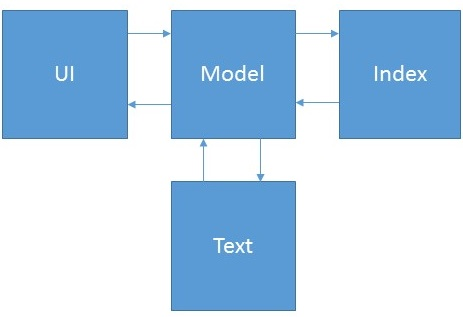
\includegraphics[]{structure}}
{\hfil\flushright{\textit{Fig 1. Interrelaci\'on de los m\'odulos}}}

\subsection{M\'odulo Interfaz de Usuario}

Es una interfaz web minimalista que cumple con los est\'andares de dise\~no para el cual el usuario solamente podr\'a interactuar
seg\'un el sistema indique.

\subsubsection{Dependencias}

Creada en {\textit{Python}} utilizando {\textit{Flask}} como {\textit{framework}} en el que las plantillas renderizadas deber\'an 
ser interpretadas debido al uso de {\textit{cookies}} en su definici\'on, entonces se requiere del m\'odulo denominado {\textit{jinja}}
para que act\'ue como int\'erprete.\\
Mientras, el dise\~no visual utiliza las clases definidas en {\textit{Bootstrap}} y los {\textit{scripts}} correspondientes, donde a
ellos se le ha a\~nadido uno propio para definir un reloj en la esquina superior derecha que ayuda a visualizar el tiempo transcurrido
entre procesos.

\subsubsection{Estructura}

Consta de cuatro rutas solamente y un enlace externo. En la barra de navegaci\'on al tope de la p\'agina est\'an enumeradas. Estas
son: ruta ra\'iz que, en caso de ser iniciada la aplicaci\'on, iniciar\'ar las {\textit{cookies}} y otras variables necesarias para la aplicaci\'on,
y en otro caso, simplemente redireccionar\'a hacia la ruta {\textbf{index}}, en ella se encuentra el grueso de la aplicaci\'on de lo cual
hablaremos a continuaci\'on, otra ruta es el "acerca" del proyecto, en el se encontrar\'an documentos relacionados con el tema como este
y, por \'ultimo, la ruta de evaluaci\'on del sistema en el que se ha descrito casos de prueba con las medidas definidas seg\'un la teor\'ia.

\subsubsection{Funcionamiento}

En la p\'agina principal se encontrar\'an los botones que indican las posibles opciones, es decir, si por ejemplo, a\'un no se ha construido
un modelo, solamente se podr\'a esperar una direcci\'on del sistema de archivos para construir uno y entonces si ya existe, se podr\'a
realizar una consulta.\\
Cada bot\'on funciona seg\'un su nombre lo indica, pero dos de ellos destacan por encima de todos ya que en ellos es donde se define
la salida v\'ia {\textit{JSON}} del sistema, los botones de construcci\'on y consulta se definen como indica la siguiente figura.

{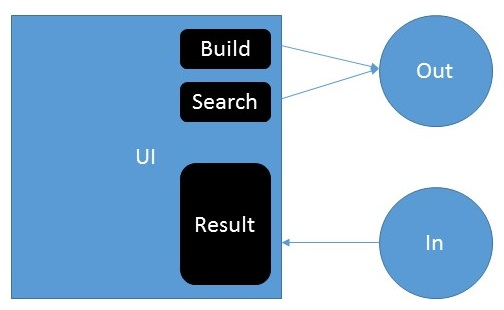
\includegraphics[]{ui}}
{\hfil\flushright{\textit{Fig 2. Entrada y salida de la interfaz de usuario}}}

\subsection{M\'odulo Procesamiento de Texto}

M\'odulo sencillo que recibe texto plano y realiza las operaciones requeridas para devolver una lista de t\'erminos v\'alidos para,
posteriormente, ser indizados.

\subsubsection{Metas alcanzadas}
El m\'odulo realiza las operaciones requeridas para el procesamiento de texto. Estas son: {\textit{stemming}} y la eliminaci\'on 
de {\textit{stopwords}} y se logran con la aplicaci\'on de la librer\'ia especificada en la secci\'on de dependencias.

\subsubsection{Dependencias}
Creada en {\textit{Python}} se apoya en su m\'odulo {\textit{NLTK}} que significa {\textit{Natural Language ToolKit}} especializado
en el procesamiento de lenguaje natural y, por consecuencia de texto, en \'el se encuentran distintos subm\'odulos, entre ellos los
necesarios son: {\textit{corpus}} y {\textit{stem}}.

\subsection{M\'odulo de \'Indices}

Es, b\'asicamente, un diccionario en forma de \'arbol en el que cada llave es un nodo que apunta hacia otra llave en el diccionario 
hasta que encuentra un nodo hoja que apunta hacia un documento.\\
Esta estructura de datos se crea en memoria y se crea seg\'un indica el m\'odulo de modelado de tal forma que evita los c\'alculos
matriciales como su definici\'on exhibe y la propagaci\'on se realiza nodo a nodo seg\'un sus aristas de peso incidiendo sobre la
activaci\'on de los mismos.

\subsubsection{Limitaciones}
El costo en memoria asciende en gran pendiente debido a la definici\'on combinatoria de los nodos y por tanto, est\'a limitado a indizar
relativamente pocos t\'erminos.

\subsubsection{Dependencias}

Creada en {\textit{Python}} no tiene ning\'un requerimento especial.

\subsection{M\'odulo de Modelado}

Est\'a creado con la intenci\'on de modelar una red neuronal para la recuperaci\'on de informaci\'on, siendo un grafo conexo y ac\'iclico tal que 
a los efectos de implementaci\'on es un \'arbol.\\
Entonces sean $X_1$, $X_2$ ... $X_n$ los t\'erminos a indizar en nuestra red neuronal, luego decimos que las combinaciones de, a lo sumo,
cinco t\'erminos conforman los nodos de la primera capa, la siguiente ser\'an las combinaciones de cuatro t\'erminos y as\'i sucesivamente
hasta llegar a los t\'erminos unitarios que representar\'an la \'ultima capa de la capa oculta hasta llegar a los nodos documentos.\\
En la siguiente figura se puede observar lo que sucede para tres t\'erminos.

{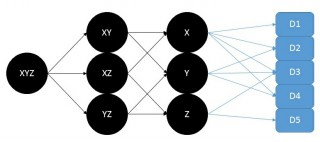
\includegraphics[]{model}}
{\hfil\flushright{\textit{Fig 3. Ejemplo de definici\'on del modelo}}}

El modelo est\'a implementado de tal forma que desde el punto de vista de la interfaz de usuario es un proceso unitario, es decir, en un ciclo de
ejecuci\'on obtiene su entrada, env\'ia y recibe lo necesario de los siguientes m\'odulos, primero procesa textos, luego crea o busca \'indices y,
finalmente, emite su salida hacia la interfaz. Esto significa que su apariencia es la siguiente:

{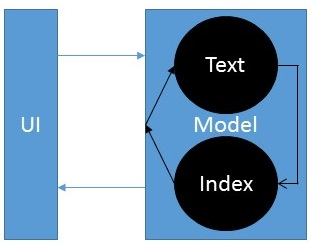
\includegraphics[]{appereance}}
{\hfil\flushright{\textit{Fig 4. Apariencia en ejecuci\'on del modelo}}}

\section{Resultados}
Adyacente al proyecto se encuentra un directorio de pruebas con pocos t\'erminos con el cual el sistema obtiene la m\'axima precisi\'on tanto en
recuperaci\'on como en el ordenamiento por relevancia, sin embargo a medida que aumenta la cantidad de t\'erminos a indizar por documentos
tanto el tiempo en ejecuci\'on como el costo en memoria se disparan exponencialmente debido al costo factorial de la combinatoria de t\'erminos
para construir los nodos.\\
Se encuentra que el sistema no es pr\'actico debido a la gran limitante computacional sin embargo, es te\'oricamente exacto ya que recubre todos
los posibles casos sobre los que un usuario promedio ejercer\'ia una acci\'on mientras que se mantiene funcional.\\
La interfaz de usuario cumple con los principios de dise\~no antes mencionados y el procesamiento de texto utiliza herramientas altamente optimizadas,
mientras la implementaci\'on del diccionario de \'indices se define seg\'un el modelo le indique, en lo que a funciones de diccionario implique es, tambi\'en,
altamente optimizada.

\section{Conclusiones}
Se encuentra un gran potencial en los sistemas de estas caracter\'isticas, especialmente aplicando el modelo de redes neuronales, con lo cual queda 
pendiente optimizar la combinaci\'on de nodos o la subdivisi\'on de consultas para obtener tales resultados para \'indices de t\'erminos mayores mientras
que se ha cumplido con los requisitos de implementaci\'on a la vez que es te\'oricamente correcto y exacto con lo cual se obtienen los mejores resultados.

\begin{thebibliography}{1}

\bibitem{mir}
Baeza-Yates, R., Ribeiro-Neto, B.:
Modern Information Retrieval.
Addison-Wesley, 1999
Longman Publishing Co., Inc., Boston, MA, USA

\bibitem{foundations}
Kasabov, Nikola.:
Foundations of Neural Networks, Fuzzy Systems and Knowledge Engineering.
MIT Press, 2002, Cambridge, MA, USA

\bibitem{paper}
Wilkinson, R., Hingston, P.:
Using the cosine measure in a neural network for document retrieval. 1991.
In Proc of the ACM SIGIR Conference on Research and Development. Chicago, USA.

\bibitem{mitra}
Mitra, B., Craswell, N.:
An Introduction to Neural Information Retrieval. 2018.
Foundations and Trends in Information Retrieval, Cambridge, UK.

\bibitem{lectures}
Kenter, T., Borisov, A., Van Gysel, C., Dehghani, M., de Rijke, M., Azarbonyad, H.:
Lectures on Neural Networks for Information Retrieval.
WSDN2018, University of Amsterdam, Netherlands.

\bibitem{conferencias}
Valle Vidal, C.:
Lectures on Artificial Neural Networks. 2009.
Universidad T\'ecnica Federico Santa Mar\'ia, Santiago, Chile

\bibitem{tesis}
Lopez, D., Navas, G.:
Dise\~no y Construcci\'on de una red neuronal de prop\'osito general.
2007, Universidad T\'ecnica Salesiana, Quito, Ecuador.

\end{thebibliography}

\end{document}